\documentclass{article}
\author{Gabriel Haruo Hanai Takeuchi - NUSP: 13671636}
\title{MAC0105 - Exercícios para 17/05}
\date{}

\usepackage[utf8]{inputenc}
\usepackage[a4paper, margin=2cm]{geometry}
\usepackage[skip=5pt]{parskip}
\usepackage{amsmath, amssymb, amsthm}
\usepackage{graphicx}


\newcommand{\set}[1]{\{#1\}}
\newcommand{\base}{\textbf{Base: }}
\newcommand{\passo}{\textbf{Passo: }}

\begin{document}
\maketitle

\section*{Exercício 31}
Prove por indução que todo polígono convexo com $n$ lados pode ser dividido em triângulos usando $n-3$ diagonais.

\begin{proof}
\textbf{Base: } Para $n=3$, diretamente é um triângulo.

\textbf{Passo: } Fixe $n \geq 4$ e suponha para $n-1$.
Vamos aumentar o polígono da H.I. (de $n-1$ lados e $n-4$ diagonais) para termos mais um triângulo interno.
Observe a imagem abaixo:
\begin{figure}[h]
    \centering
    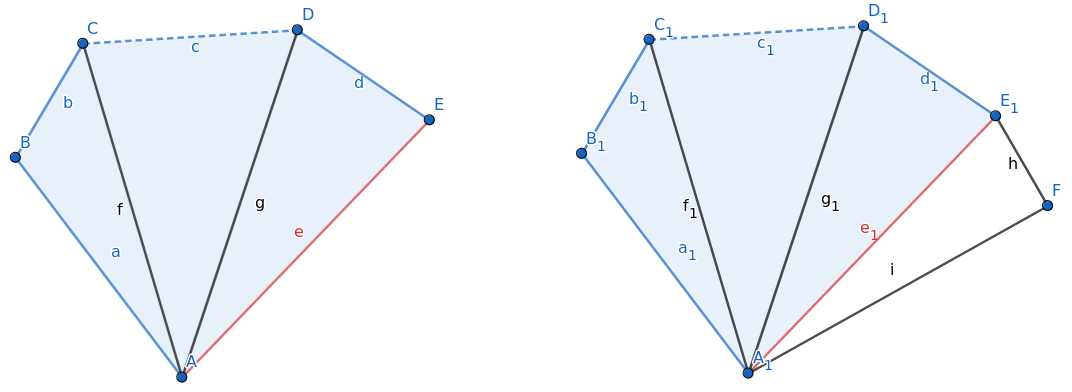
\includegraphics[width=0.8\textwidth]{triangulos.png}
\end{figure}

Adote o vértice que espana todas as diagonais como vértice $A$.
Ao criar uma nova aresta de $A$ (no caso $AF$) e criar outra aresta $EF$, o antigo lado vermelho tornou-se uma diagonal.
Logo, temos um novo polígono com $n$ lados, $n-3$ diagonais e dividido em triângulos, como queríamos.

\end{proof}

\section*{Exercício 33}
Prove que para inteiro $n \geq 10$ temos que $100n \leq 2^n$.
\begin{proof}
Vamos provar por indução em $n$.

\textbf{Base: } Para $n=10$, diretamente $100\cdot 10 = 1000 \leq 1024 = 2^{10}$.

\textbf{Passo: } Fixe $n \geq 11$ e suponha a H.I. para $n-1$.

Por hipótese, temos que 
\[
    100(n-1) \leq 2^{n-1} \implies 100(n-1) \cdot 2 \leq 2^{n-1} \cdot 2
    \implies 200n - 200 \leq 2^n \; .
\]
Seria muito bom se, para $n \geq 11$, $100n \leq 200n - 200$. Vamos verificar:
\[
    100n \leq 200n - 200 \iff n \geq 2 \; .
\]
Logo, se é satisfeito para $n \geq 2$, também é para $n \geq 11$.

Portanto, temos finalmente que 
\[
    100n \leq 200n - 200 \leq 2^n \implies 100n \leq 2^n \;
\]
, como queríamos.
\end{proof}

\section*{Exercício 35}
Uma árvore é um grafo conexo com $n$ vértices e $n-1$ arestas.
Uma folha de uma árvore é um vértice de grau 1.
Um caminho é uma árvore com exatamente 2 folhas.
Prove os seguintes resultados:
Seja $T$ uma árvore com $n$ vértices. Então,

(a) $T$ tem pelo menos 2 folhas (por indução);
\begin{proof}
Vamos provar por indução.

\base Para $n=2$, temos apenas 2 vértices com 1 aresta os ligando.
Diretamente, ambos os vértices têm grau 1.

\passo Fixe $n \geq 3$ e suponha para $n-1$.
Suponha um árvore $T'$ com $n-1$ vértices e $n-2$ arestas que tenha pelo menos 2 folhas.
Queremos uma árvore $T$ com $n$ vértices e $n-1$ arestas que também tenha pelo menos 2 folhas.
Note, devemos adicionar exatamente 1 vértice e 1 aresta em $T'$ para podermos ter $T$.

Atente-se que, como uma árvore é um grafo conexo, então a adição de um vértice $v$ deve ser seguida de uma aresta em $v$, e portanto $v$ tem grau 1.
Vamos separar a adição de um vértice em casos:

\textit{Caso I: ligar um novo vértice a um vértice não-folha}

Diretamente, ao conectar um novo vértice a um já existente de grau maior que 1, teremos pelo menos 3 vértices de grau maior que 1.

\textit{Caso II: ligar um novo vértice a um vértice folha}

Suponha que $v_f$ seja uma folha em $T'$.
Ao conectar um novo vértice $v_n$ a $v_f$, logo $v_f$ não é mais folha.
Entretanto, $v_n$ se torna uma nova folha, assim mantendo a condição de pelo menos 2 folhas.

Em ambos os casos, a nova árvore $T$ ainda mantém o mínimo de 2 folhas, como queríamos.
\end{proof}

(b) existe exatamente um caminho entre quaisquer dois vértices de T .
\begin{proof}
Vamos provar por indução.

\base Para $n=2$, diretamente há um único caminho entre os vértices.

\passo Fixe $n \geq 3$ e suponha uma árvore $T'$ com $n-1$ vértices tal que existe um único caminho entre dois vértices de $T$.

Novamente, iremos adicionar 1 vértice $v_n$ e 1 aresta que liga $v_n$ a algum nó de $T'$.

Seja $v_x$ um vértice qualquer de $T'$.
Ao conectarmos $v_n$ e $v_x$, então diretamente temos um único caminho entre eles.
Note que, por hipótese, existe um único caminho entre $v_x$ e qualquer outro nó de $T'$.
Se temos um único caminho entre $v_n$ e $v_x$ e temos um único caminho entre $v_x$ e qualquer outro nó de $T'$, então temos um único caminho entre $v_n$ e qualquer outro nó de $T'$.

Logo, temos uma nova árvore $T$ com $n$ vértices e exatamente um único caminho entre qualquer par de vértices, como queríamos.
\end{proof}

\section*{Exercício 37}
Prove por indução que $F_n \leq 2n$ para todo inteiro positivo $n$, em que $F_n$ é o $n$-ésimo número de Fibonacci.
\begin{proof}
Vamos provar por indução em $n$.

\base Para $n=1$, $F_1 = 1 < 2 = 2 \cdot 1 = 2n$.
Para $n=2$, $F_2 = 2 < 4 = 2 \cdot 2 = 2n$.

\passo Fixe $n \geq 3$ e suponha para $n-1$ e $n-2$.

\begin{align*}
    F_{n-1} &\leq 2(n-1) \\
    F_{n-1} + F_{n-2} &\leq 2n-2 + F_{n-2} \\
    F_n &\leq 2n-2 + F_{n-2} \\
\end{align*}
Por hipótese, $F_{n-2} \leq 2(n-2) = 2n - 4$. Logo, temos o resultado
\begin{align*}
    F_n &\leq 2n-2 + F_{n-2} \leq 2n-2 + 2n-4 = 4n - 6 = 2(n-3) \leq 2n
\end{align*}
, como queríamos.
\end{proof}

\end{document}